\documentclass{standalone}
\usepackage{tikz}
\usepackage{pgfplots}
\pgfplotsset{width=32cm,height=18cm,compat=1.3}
\pgfplotsset{every tick label/.append style={font=\Huge}}
\usepackage{filecontents}

\usetikzlibrary{patterns}

\definecolor{citrine}{rgb}{0.89, 0.82, 0.04}

\begin{document}
	\centering
		\vspace{1.5em}
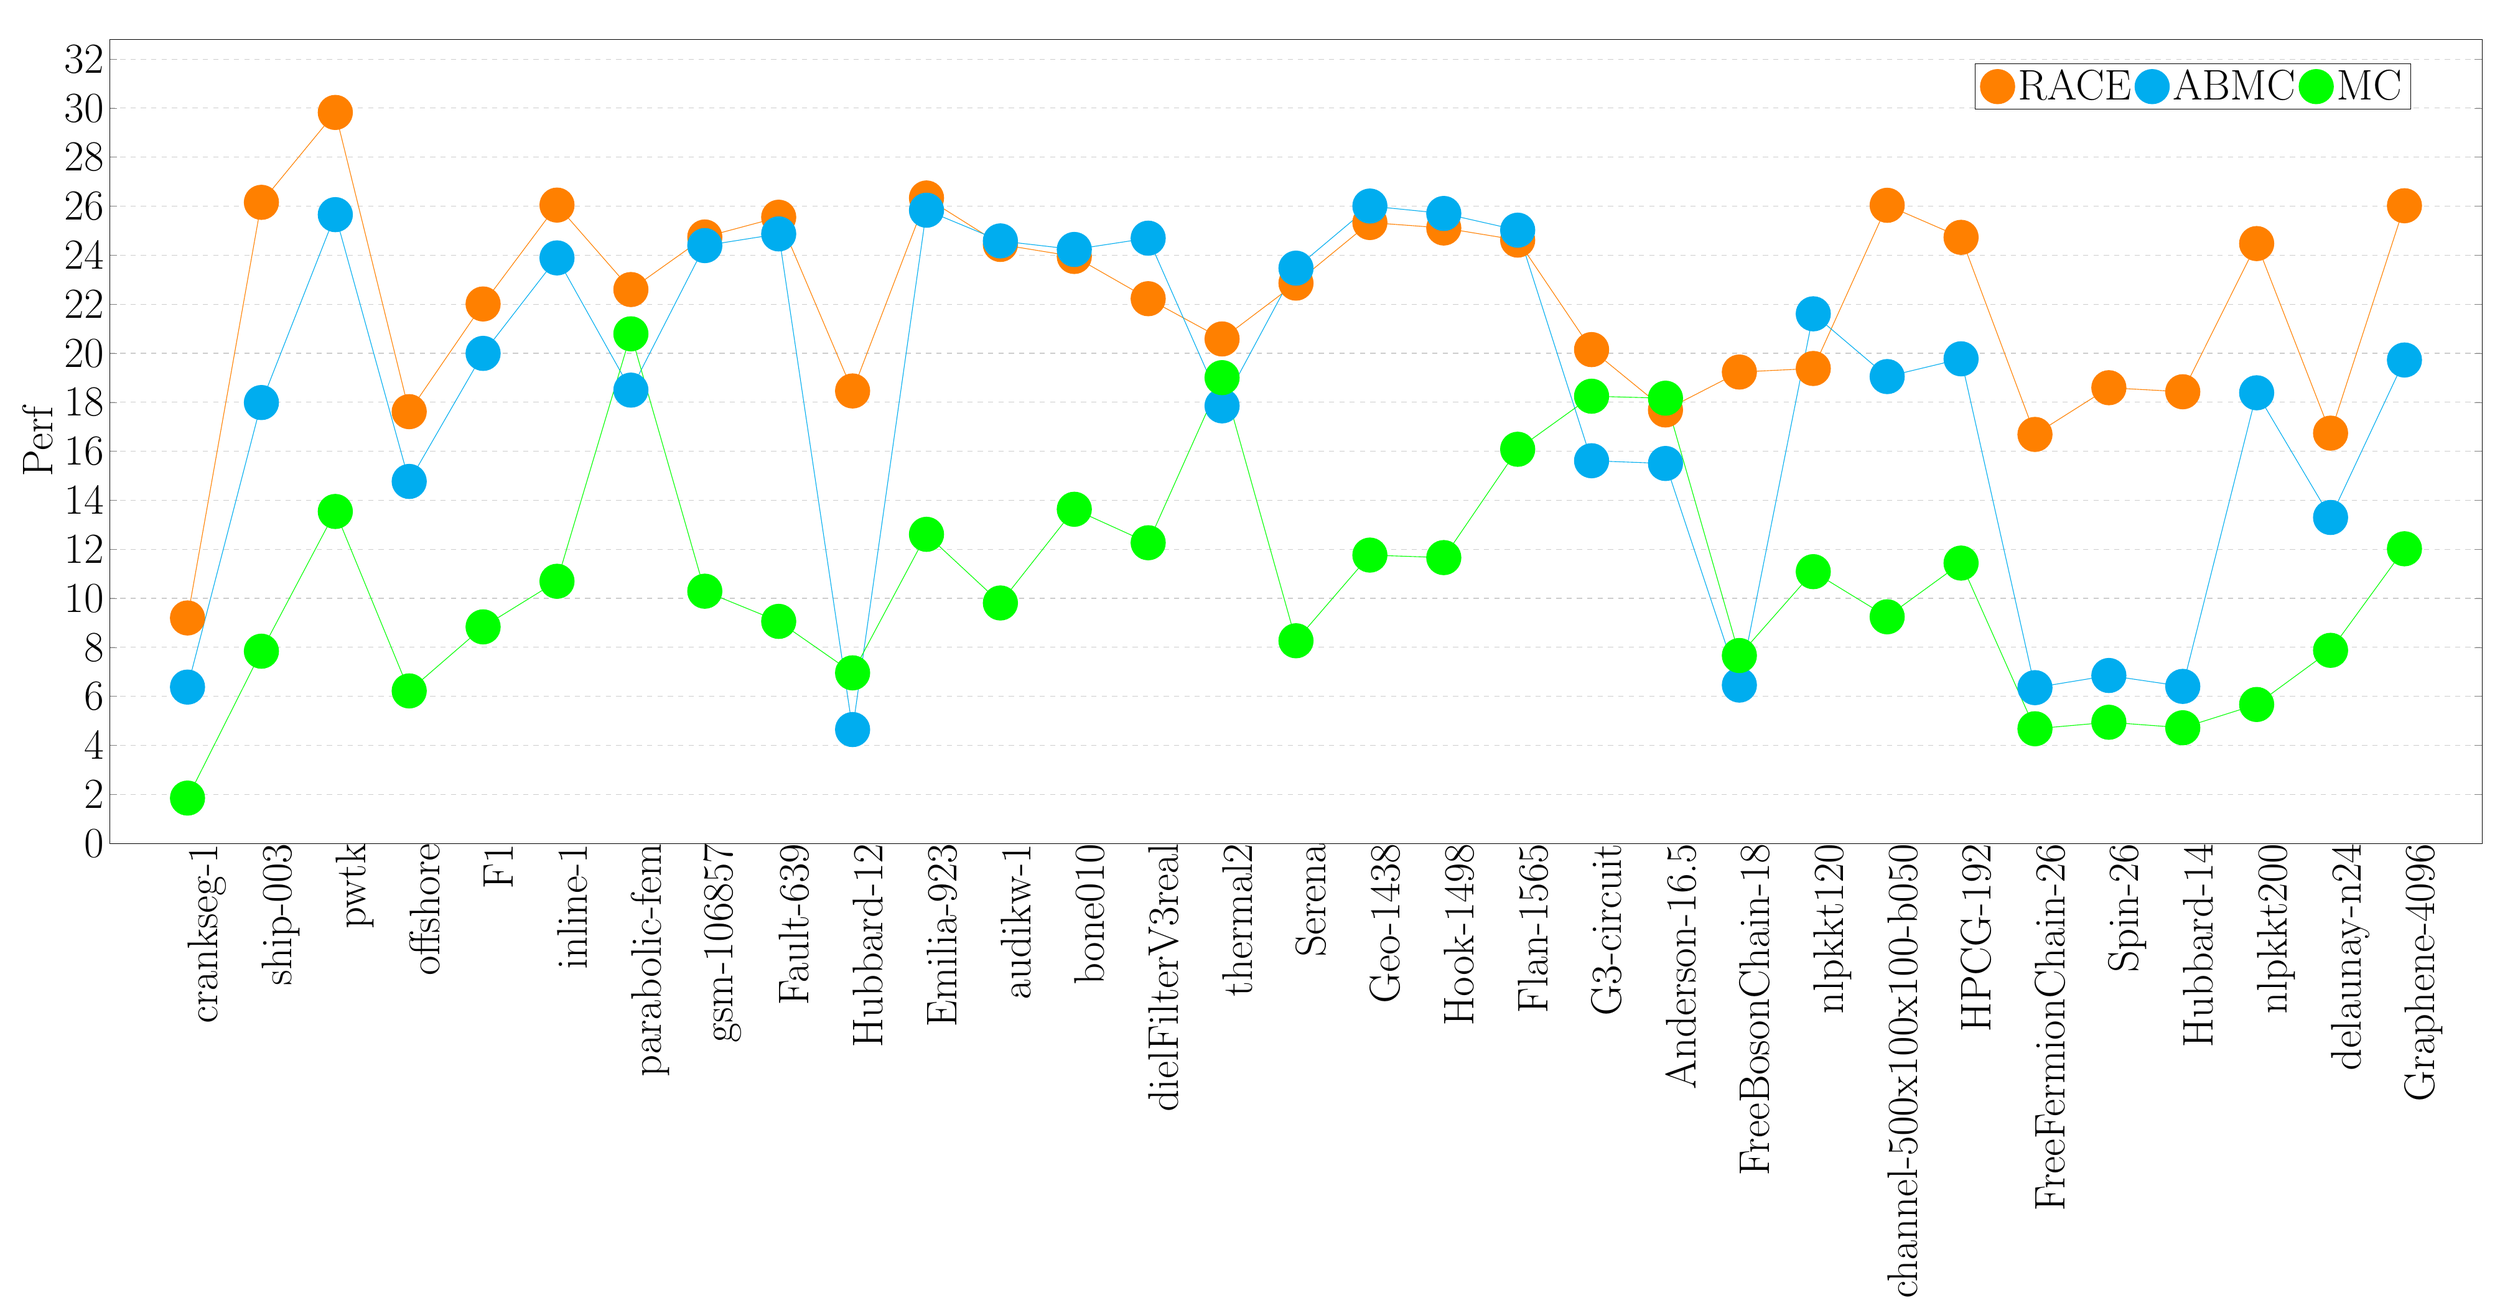
\begin{tikzpicture}
		%	\node at (13.25,15) {\LARGE{}};
			\begin{axis}[
		%	xmin=0.25, xmax=7.25,
			ymin=0, %ymax=3.25,
			xtick={1, 2, 3, 4, 5, 6, 7, 8, 9, 10, 11, 12, 13, 14, 15, 16, 17, 18, 19, 20, 21, 22, 23, 24, 25, 26, 27, 28, 29, 30, 31},
		%	ytick={0,0.5,1,1.5,2,2.5,3},
			xticklabels={crankseg-1, ship-003, pwtk, offshore, F1, inline-1, parabolic-fem, gsm-106857, Fault-639, Hubbard-12, Emilia-923, audikw-1, bone010, dielFilterV3real, thermal2, Serena, Geo-1438, Hook-1498, Flan-1565, G3-circuit, Anderson-16.5, FreeBosonChain-18, nlpkkt120, channel-500x100x100-b050, HPCG-192, FreeFermionChain-26, Spin-26, Hubbard-14, nlpkkt200, delaunay-n24, Graphene-4096},
			width  = 50cm,
			height = 18cm,
			major x tick style = transparent,
			%	minor ytick={1, 5, 10, 15, 20, 25, 30 ,35,40},
			grid = minor,	
			%add_bar_commands
			ymajorgrids = true,
			grid style={dashed, gray!40},
			ylabel = {\Huge{Perf}},
		%	symbolic x coords={Graphene-2048-2048, Graphene-4096-4096, Spin-24-24-24},
			x tick label style={rotate=90, anchor=north east, inner sep=0mm, font={\Huge}},
			tick label style={font={\Huge}},
			scaled y ticks = false,
			enlarge x limits=0.035,
			legend cell align=left,
			legend style={font=\Huge},
			legend columns=-1,
			legend style={
				%at={(1,1.05)},
				%anchor=south east,
				%column sep=1ex,
				legend pos=north east
			},
			%spl_legend_code
			title= {\Huge\scalebox{1.5}{{}}}
			]

\addplot[ mark=*, mark size=10pt, mark options={orange}, draw=orange ] plot coordinates{(1,9.198385) (2,26.157869) (3,29.826118) (4,17.616318) (5,22.010906) (6,26.045767) (7,22.599533) (8,24.743882) (9,25.550477) (10,18.461244) (11,26.335494) (12,24.439999) (13,23.949504) (14,22.225418) (15,20.583243) (16,22.860712) (17,25.334251) (18,25.110342) (19,24.616822) (20,20.148802) (21,17.685403) (22,19.233015) (23,19.378427) (24,26.037220) (25,24.729376) (26,16.687338) (27,18.593029) (28,18.428171) (29,24.475084) (30,16.739471) (31,26.018944)};
\addplot[ mark=*, mark size=10pt, mark options={cyan}, draw=cyan ] plot coordinates{(1,6.377376) (2,17.988623) (3,25.655813) (4,14.769430) (5,19.994491) (6,23.890335) (7,18.494966) (8,24.392305) (9,24.869456) (10,4.644608) (11,25.836294) (12,24.583953) (13,24.234832) (14,24.695893) (15,17.852862) (16,23.471796) (17,26.006676) (18,25.703345) (19,25.021309) (20,15.613656) (21,15.501743) (22,6.459218) (23,21.608993) (24,19.048035) (25,19.772437) (26,6.354355) (27,6.850660) (28,6.406094) (29,18.386339) (30,13.299116) (31,19.724410)};
\addplot[ mark=*, mark size=10pt, mark options={green}, draw=green ] plot coordinates{(1,1.847996) (2,7.841710) (3,13.543612) (4,6.221272) (5,8.834178) (6,10.694937) (7,20.792456) (8,10.290035) (9,9.058860) (10,6.958355) (11,12.611237) (12,9.809832) (13,13.633760) (14,12.266884) (15,19.004321) (16,8.267427) (17,11.763698) (18,11.661271) (19,16.081831) (20,18.246749) (21,18.165817) (22,7.665613) (23,11.087210) (24,9.245484) (25,11.437391) (26,4.677296) (27,4.942705) (28,4.717942) (29,5.667727) (30,7.877398) (31,12.021101)};
	%addplot cmd

	\legend{RACE, ABMC, MC}

	\end{axis}			
\end{tikzpicture}

\end{document}

